%%%%%%%%%%%%%%%%%%%%%%%%%%%%%%%%%%%%%%%%%%%%%%%%%%%%%%%%%%%%%%%%%%%%%%%%
%                                                                      %
%     File: Thesis_Implementation.tex                                  %
%     Tex Master: Thesis.tex                                           %
%                                                                      %
%     Author: Andre C. Marta                                           %
%     Last modified :  2 Jul 2015                                      %
%                                                                      %
%%%%%%%%%%%%%%%%%%%%%%%%%%%%%%%%%%%%%%%%%%%%%%%%%%%%%%%%%%%%%%%%%%%%%%%%

\chapter{Algorithm}
\label{chapter:algorithm}

Our algorithm (refered to as CRSH from now on) creates a Coherent Ray-Space Hierarchy that takes advantage of the properties of highly coherent rays to render photo-realistic images.
It consists of seven major steps (see Figure~\ref{fig:crsh}). 

We use the GPUs rasterizer to compute the primary rays and then output the necessary information to create the initial batch of secondary rays. We then sort those rays, create the hierarchy and traverse it. The final step consists in intersecting the bottom-level of the hierarchy with the geometry and accumulating shading.

In each frame steps 1 and 2 are executed only once while steps 3 through 7 are executed once per ray batch. A ray batch can consist of any combination of shadow rays, reflection rays or refraction rays. This means that we can use batches that only contain shadow rays, only reflection rays, only refraction rays or any combination of the aforementioned types.

\begin{figure}[!htb]
    \centering
    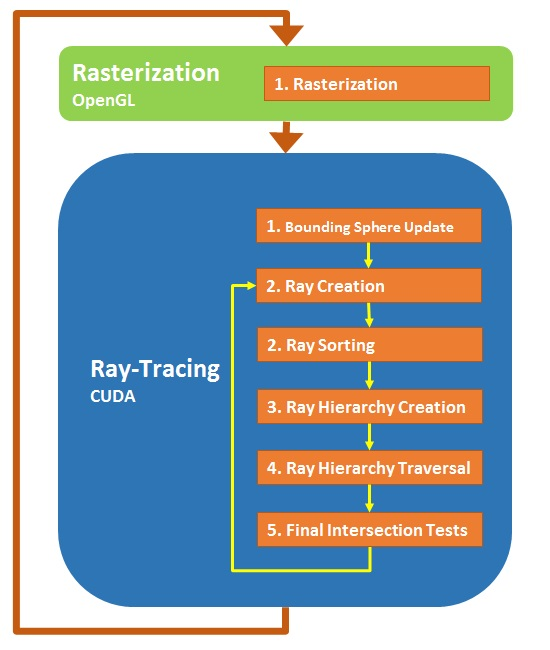
\includegraphics[width=0.45\textwidth]{Images/Overview}
    \caption{\label{fig:crsh}Coherent Ray-Space Hierarchy Overview.}
\end{figure}

%%%%%%%%%%%%%%%%%%%%%%%%%%%%%%%%%%%%%%%%%%%%%%%%%%%%%%%%%%%%%%%%%%%%%%%%
\section{Rasterization}
\label{section:algorithm-rasterization}

Rasterization is the first step of the algorithm. There was an ongoing urban legend that Rasterization and Ray-Tracing are polar opposites and that a choice has to be made between these two techniques. This is not true at all. Although Rasterization solves the rendering problem conversely vs Ray-Tracing (i.e. projecting primitives to the screen, vs projecting rays backwards to the primitives in the scene), one can complement the other. 
The first set of rays, the primary rays, does not convey any of the global illumination effects that Ray-Tracing is well suited to achieve, such as Shadows, Reflections and Refractions. This means that Rasterization can convey similar visual results to tracing the primary rays, while being extremely faster and optimized in the graphics hardware. Supplementing the Rasterization of primary rays with the Ray-Tracing of secondary rays can get us the benefits from both techniques: the efficiency of Rasterization and the global illumination effects from Ray-Tracing.

\medskip

In order to combine both techniques the output from the fragment shaders used to rasterize the scene must be more than just the traditional fragment colors. We need to create different render targets according to the information we want to store. In our case we output the fragment diffuse and specular properties, the fragment position and the fragment normal. In our implementation the fragment shader outputs 4 different textures containing four 32 bit floats per pixel each. These textures are generated with OpenGL/GLSL and are then sent to CUDA to create the first level of secondary rays.

\medskip

The first pair of textures, the diffuse and specular properties textures, are used to calculate the shading of the primary rays. Although the primary rays are computed in the rasterizer, it is also important to note that after every batch of rays (primary or secondary) we need to trace shadow rays to determine the shading of those rays. We could store the triangle ID instead of the diffuse and specular properties but we chose the latter two instead. We store these two values instead of the triangle IDs so that we can prevent memory accesses and calculations. If we chose to output the triangle ID this would require us to calculate the triangle ID in the context of the scene (the rasterizer computes one object at a time therefore an extra step would be necessary). It would also require three different global memory accesses (the triangle IDs texture, the diffuse properties array and the specular properties array) compared to the two accesses if we just access the material values directly. The size of the two textures are also negligible when compared to the total memory requirements of the algorithm, therefore there is no reason not to use these two textures instead of one that contains the triangle IDs.

\medskip

The second pair of textures, the fragment position and normal textures, contain the information necessary to calculate the secondary rays. These include the shadow, reflection and refraction rays. However it is important to note that to calculate the shadow rays it is only necessary to output the fragment position, since the shadow ray directions are determined by the light and fragment positions. This means that the fragment normal is only needed for the reflection and refraction rays.

%%%%%%%%%%%%%%%%%%%%%%%%%%%%%%%%%%%%%%%%%%%%%%%%%%%%%%%%%%%%%%%%%%%%%%%%
\section{Ray-Tracing}
\label{section:algorithm-ray-tracing}

\subsection{Bounding Volume Creation}

Although this is a pre-processing step it makes sense to mention it now since in the following step we will update the object-based bounding spheres. We pre-compute the minimal bounding sphere of the object meshes, using an implementation based on \cite{Gartner99}s algorithm. It is important to use the minimal bounding spheres because these spheres will be used later on in the algorithm (in the hierarchy traversal step) to cull potential intersections in an early phase and thus reduced the total number of intersection tests computed. Since these are all pre-processed they have no impact on render time performance.

\subsection{Bounding Volume Update}

In this step we update the object bounding spheres according to the transformations being applied to the object they envelop (e.g. translation, rotation, scale). Since we only update the center and the radius there is no need to recalculate the bounding spheres in each frame (the transformations do not invalidate the bounding spheres themselves).

\subsection{Secondary Ray Creation and Indexing}

After the updating the bounding spheres we need to create the secondary rays. This step includes both the creation and the indexing of said rays. This step can be executed right after the rasterization step or after the final intersections step, depending on the ray-tracing depth being used. The ray index will be used later on in the algorithm in the sorting step. Since this is the first of the repeatable steps in our algorithm we will present both cases, the one where the rays are created right after the rasterization step as well as the one where rays are created after processing a ray batch.

\subsubsection{Secondary Ray Creation}

We will now present the formulas used to calculate the secondary rays. After the Rasterization step they are created by using the textures that contain the fragment positions and normals. If this is executed after processing another ray batch then the rays are created using the information obtained from the final intersection tests step (this information is still the fragment position and normals, it only means that the rays are created right after the shading step). 

\medskip

For that reason, the formulas are generic enough so that they can be used for both steps without any need for modifications. After this step it is irrelevant if we are processing the first batch of secondary rays or not since they are all processed in the same way, up until the final intersection tests.

\pagebreak

The following formula is used to create the shadow rays:

\begin{equation}
    \mathlarger{o = l}
\end{equation}

\begin{equation}
    \mathlarger{\vec{d} = \frac{ \vec{p} - \vec{o} }
                               {|\vec{p} - \vec{o}|}}
\end{equation}                 

\begin{align*}
    \textbf{o} = Origin, \mathbf{\vec{d}} = Direction,                     
    \textbf{p} = Fragment Position,
    \textbf{l} = Light Position\\
\end{align*}
            
The following formula is used to create the reflection rays:

\begin{equation}
    \mathlarger{o = p}
\end{equation}

\begin{equation}
    \mathlarger{\vec{d} = \vec{i} - 2 \times \vec{n} \times (\vec{n} \cdot \vec{i})}
\end{equation}

\begin{align*}
    \textbf{o} = Origin, \mathbf{\vec{d}} = Direction,                     
    \textbf{p} = Fragment Position,
    \textbf{i} = Incident Ray Direction\\
\end{align*}

% return i - 2.0f * n * dot(n,i);

The following formula is used to create the refraction rays:

\begin{equation}
    \mathlarger{o = p}
\end{equation}  

\begin{equation}
    \mathlarger{k = 1 - ri^{2} \times (1 - (\vec{i} \cdot \vec{n})^{2})}
\end{equation}  

\begin{equation}
    \mathlarger{\vec{d} = \vec{i} \times ri - \vec{n} \times (ri \times (\vec{i} \cdot \vec{n}) + \sqrt{k})}
\end{equation}  

\begin{align*}
    \textbf{o} = Origin, \mathbf{\vec{d}} = Direction,                     
    \textbf{p} = Fragment Position,
    \textbf{i} = Incident Ray Direction,
    \textbf{ri} = Refraction Index\\
\end{align*}
            
% float k = 1.0f - pow(ior,2) * (1.0f - pow(dot(i, n),2));
% return i * ior - n * (ior * dot(i, n) + sqrtf(k));       

\pagebreak

\subsubsection{Secondary Ray Indexing}

We create an index for each individual ray in order to sort the secondary rays in the following steps. We use a different hashing function for each type of ray (see Figures~\ref{fig:srh}, ~\ref{fig:rrh}). Since each ray consists of an origin and a direction it would be straightforward to simply use these two parameters to create our hash. However for shadow rays it is sufficient to use the index of the light source to which it belongs and its direction. This is only possible however if we invert the origin of the shadow ray so that it originates at the light source rather than the originating fragment. To further reduce the size of the hash keys we convert the ray direction into spherical coordinates \cite{GraphicGems5} and store both the light index and the spherical coordinates into a 32 bit integer, with the light index having the higher bit-value such that the shadow rays are sorted according to the light source a priori.

\medskip

\begin{figure}[!htb]
    \centering
    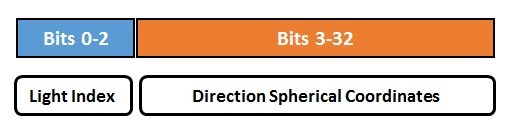
\includegraphics[scale=0.85]{Images/Shadow_Hash}
    \caption{\label{fig:srh}Shadow Ray Hash.}
\end{figure}

The Reflection and Refraction rays are also converted to spherical coordinates. However in this case the ray origin is used in the hash instead of being discarded, given that these rays are not as coherent in regards to their origin. These rays are only coherent locally, for example if they are all originating from the same area in the same object, unlike shadow rays which have the same origin for each light source. This also means that the indexing step is extremely important for our algorithm because if we can sort these rays optimally we will also get an optimal hierarchy, leading to a greatly reduced number of intersection tests.

\begin{figure}[!htb]
    \centering
    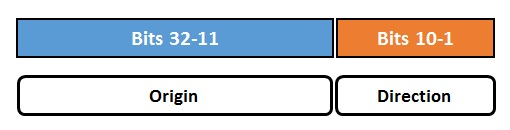
\includegraphics[scale=0.85]{Images/Reflection_Hash}
    \caption{\label{fig:rrh}Reflection and Refraction Ray Hash.}
\end{figure}

\subsubsection{Secondary Ray Trimming}

Once the secondary rays are created and indexed, we have four arrays, the ray array that contains the generated secondary rays, two arrays that contain the ray keys (the indices's we calculated) and the ray values (the rays position in the ray array) and a final array with head flags which indicate if there is a ray in the corresponding position within the key-value arrays, where we store either a 0 or a 1, indicating if there is a ray or not, respectively.

\medskip

Using the information from the head flags array we then run a trimming operator on the key-value arrays (see Figure~\ref{fig:at}). This is done by first applying an inclusive scan operator \cite{Merrill09} on the head flags array, which gives us the number of positions that each pair needs to be shifted to the left. This is done in order to trim the arrays \cite{GPUGems2}. This is an extremely important step for parallel programming since by doing this we can deduce the number of rays (by checking the last position of the scan array) as well as having all the rays that need to be processed in adjacent positions, meaning there will be no thread processing the empty spaces in the arrays.

\begin{figure}[!htb]
    \centering
    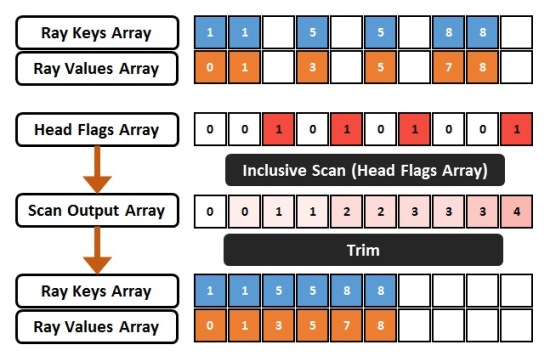
\includegraphics[scale=0.75]{Images/Array_Trimming}
    \caption{\label{fig:at}Array Trimming}
\end{figure}

\subsection{Secondary Ray Compression}

After trimming the secondary rays we used a compression-sorting-decompression scheme, expanding on prior work by Garanzha and Loop \cite{Garanzha10}. The compression step exploits the local coherency of rays. Even for secondary rays, the bounces generated by two adjacent rays have a good chance of being coherent (i.e. a sphere reflecting rays around an area, see Figure~\ref{fig:rr}). 

\begin{figure}[!htb]
    \centering
    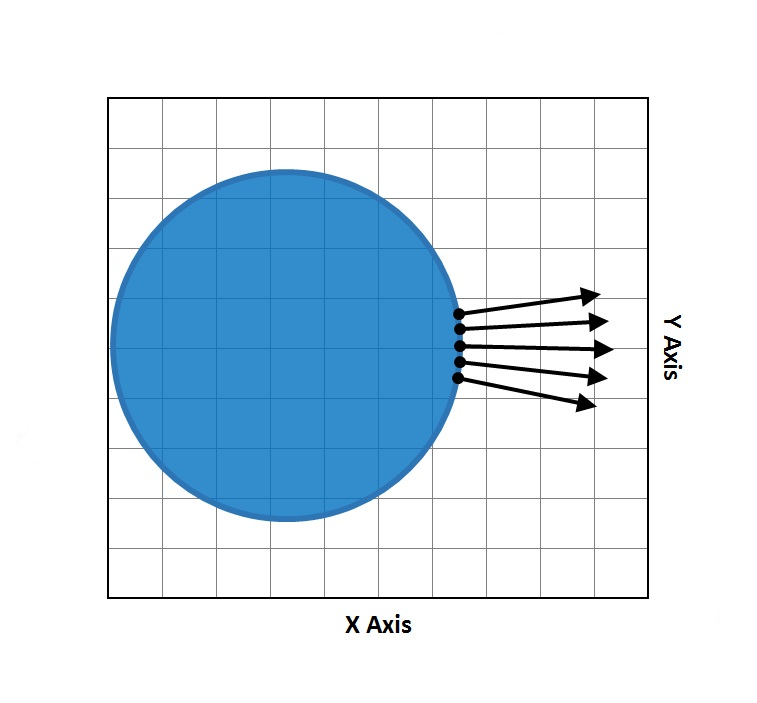
\includegraphics[scale=0.325]{Images/Ray_Reflection}
    \caption{\label{fig:rr}Ray Reflection}
\end{figure}

This coherency means that these rays can end up having the same hash value. Given these rays with the same hashes, we compress the ray key-value pairs into chunks, minimizing the number of pairs that need to be sorted. To compress the pairs we utilize a head flags array with the same size as the key-value pair array, initializing it with $0$s in every position and inserting $1$s into positions in which the key (hash) of the corresponding pair differs from the previous pair. After populating the head flags array we apply an inclusive scan operator on it \cite{Merrill09}. By combining the head flags array with the scan output array we create the chunk keys, base and size arrays, which contain the hash, starting index and size of the corresponding chunks (see Figure~\ref{fig:rcc}). The chunk keys are represented in different colors at the image below. The chunk base array represents the original position of the first ray in the chunk while the chunk size array represents the size of the chunk, needed for the ray array decompression.

\begin{figure}[!htb]
    \centering
    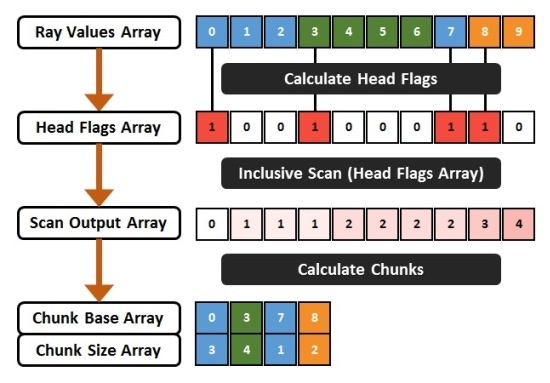
\includegraphics[scale=0.75]{Images/Ray_Compression}
    \caption{\label{fig:rcc}Ray Compression into Chunks}
\end{figure}

It is important to note that even though there are only the chunk base and size arrays in Figure~\ref{fig:rcc} the compression step also creates two more arrays, the chunk keys array (that contains the indices's of the corresponding rays) and the chunk values array (that contains the position of the corresponding chunk key, initially a sorted array). These arrays will be used for the sorting step.

\subsection{Secondary Ray Sorting}

After compressing the rays we have the chunk base and size arrays that contain the necessary information to reconstruct the initial rays array and the chunk keys and values arrays that contain the necessary information for the sorting process. With the latter two we apply a radix sort \cite{Merrill11} (see Figure~\ref{fig:rs}) and obtain two sorted arrays containing the ray keys and values. The ray keys array is irrelevant after this stage since it was only necessary to sorting the ray values array.

\begin{figure}[!htb]
    \centering
    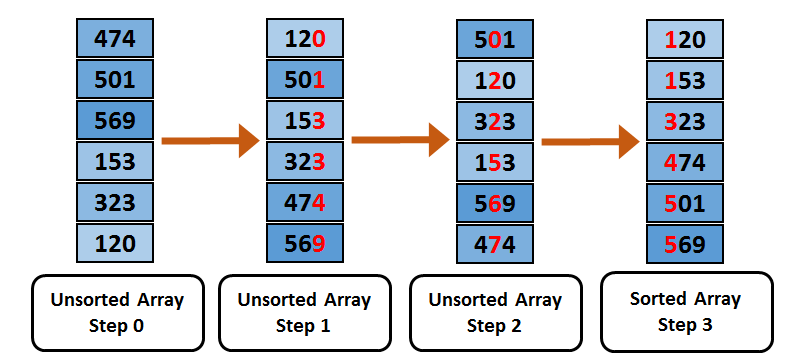
\includegraphics[scale=0.75]{Images/Radix_Sort}
    \caption{\label{fig:rs}Radix Sort}
\end{figure}

\subsection{Secondary Ray Decompression}

Finally the chunk decompression begins with the creation of a skeleton array with the same size as the sorted chunk base and size arrays. This skeleton array contains the size of the sorted chunks in each position. Next we apply an exclusive scan operator on the skeleton array, originating a scan array. This scan array gives us the starting positions positions of each chunks in the sorted ray key and value arrays. After creating these two arrays (the skeleton and scan arrays) we fill the sorted ray array. We start in the position indicated in the scan array and finish after filling the number of rays indicated in the skeleton array. Although Figure~\ref{fig:rd} has the chunk size array with the exact same values as the skeleton array its important to note that this is simply a representation for easier understanding since at this point we do not have a sorted chunk size array but instead a sorted values array that when combined with the chunk size array we created when we compressed the rays into chunks will give us the sorted chunk sizes.

\begin{figure}[!htb]
    \centering
    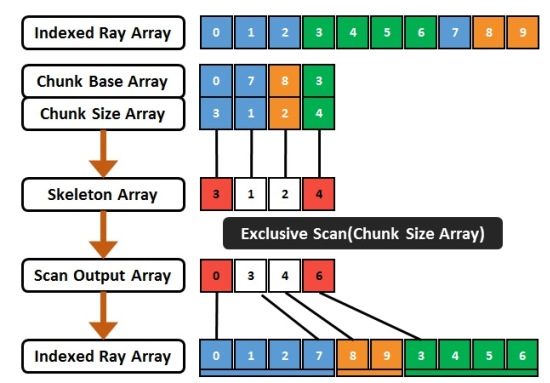
\includegraphics[scale=0.75]{Images/Ray_Decompression}
    \caption{\label{fig:rd}Ray Decompression from Chunks}
\end{figure}

To summarize these last three sections, we first compressed the rays into chunks, we sort the chunks are finally decompressed the sorted chunks (see Figure~\ref{fig:so}).   

\begin{figure}[!htb]
    \centering
    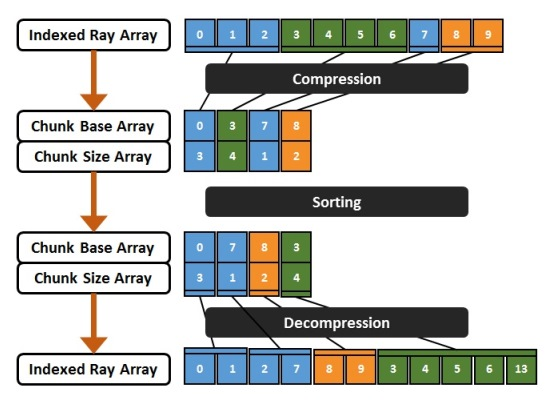
\includegraphics[scale=0.90]{Images/Sorting_Overview}
    \caption{\label{fig:so}Sorting Overview}
\end{figure}

\subsection{Hierarchy Creation}

With the sorted rays we can now create the ray hierarchy. Since the rays are now sorted coherently the hierarchy will be much tighter in its lower levels, giving us a smaller number of intersection candidates as we traverse further down the hierarchy.

\medskip

Each node in the hierarchy is represented by a sphere and a cone (see Figures~\ref{fig:bc}, \ref{fig:bs}).
The sphere contains all the nodes ray origins while the cone contain the rays themselves (see Figure~\ref{fig:cru}). This structure is stored using eight floats: the sphere center and radius (four floats) and the cone direction and spread angle (four floats). The construction of the hierarchy is done in a bottom-up fashion. Thus we start with the leaves, with spheres of radius $0$ and a cone with spread angle equal to $0$. These leaves correspond to the sorted rays. The upper levels of the hierarchy are created by calculating the union of the child nodes. The number of children combined in each node can also be parametrized. 

%\medskip
%It is also important that each ray knows the pixel that it corresponds to. After the sorting step rays are not in their %original order so we need a way to map rays back to the screen pixels. This is easily solved since the original %position of the ray in the ray array maps directly to the corresponding pixel.

\medskip

It is important to take into consideration that since the hierarchy is not tied directly to the geometry positions in the scene it does not matter for hierarchy creation whether the scene is dynamic or static. This means that creating the scene with a moving object does not impact performance at all. What does impact performance is the number of secondary rays generated and this can be affected by the number of objects in the screen (more specifically the number of fragments that each object creates, which directly correlates to the number of secondary rays generated). The only thing that does matter directly is the number of bounces of each ray, meaning that if there are more pixels occupied in the screen, the hierarchy will forcibly have more nodes.

\medskip

\begin{figure}[!htb]
    \centering
    
    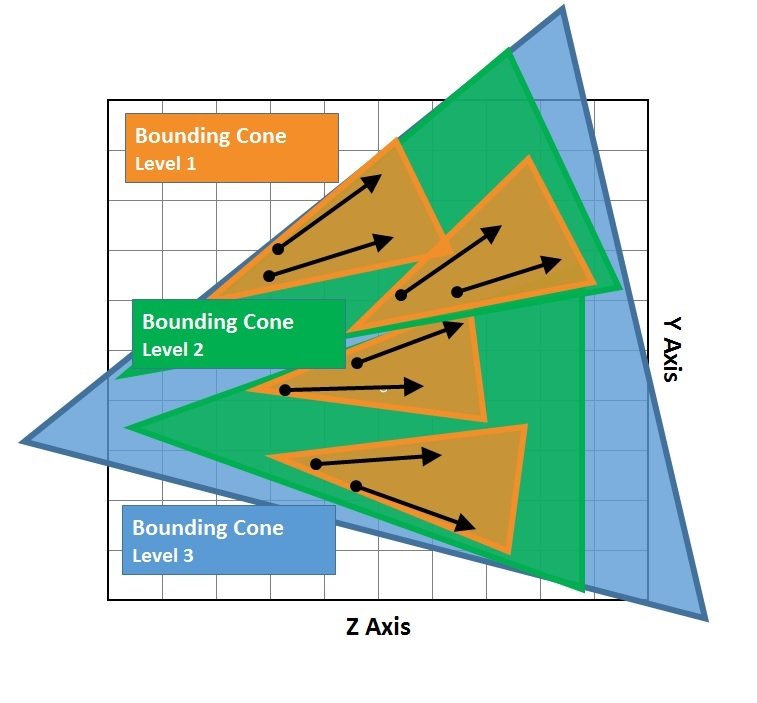
\includegraphics[scale=0.30]{Images/Bounding_Cone}
    \caption{\label{fig:bc}Bounding Cone - 2D View}

    \vspace{2.5pt}

    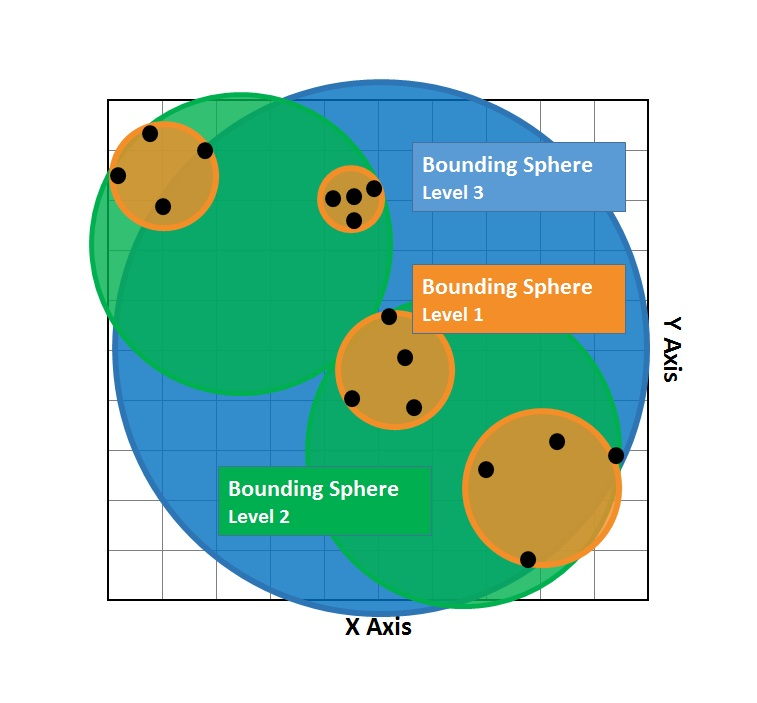
\includegraphics[scale=0.30]{Images/Bounding_Sphere}
    \caption{\label{fig:bs}Bounding Sphere - 2D View}
\end{figure}

\begin{figure}[!htb]
    \centering
    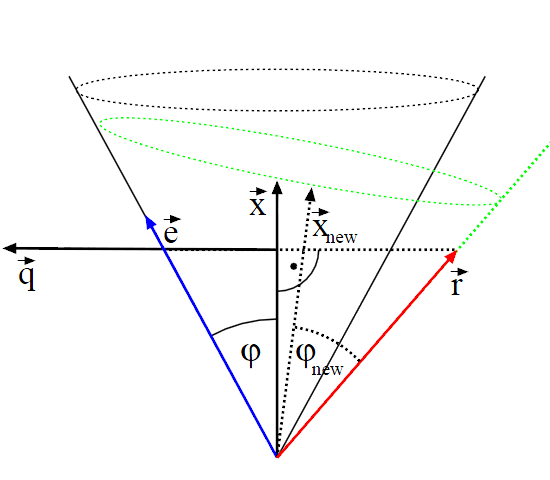
\includegraphics[scale=0.40]{Images/Cone_Union}
    \caption{\label{fig:cru}Cone-Ray Union - 2D View. \small{courtesy of \cite{Szecsi06}}.}
\end{figure}

We will now present the formulas used for the creation of each individual node. For the first level of nodes we use a different formula for the creation of the cones. This is done because the first level is a particular case. The leaves of the hierarchy are simply rays therefore it is more efficient to used a different formula ir order to create more compact cones \cite{Szecsi06}.

\medskip

The following formulas are used to create the first level nodes:

\begin{equation}
    \mathlarger{\vec{q} = \frac{ (\vec{x} \cdot \vec{r}) \cdot \vec{x} - \vec{r} }
                                {|(\vec{x} \cdot \vec{r}) \cdot \vec{x} - \vec{r}|}}
\end{equation}

\begin{equation}
    \mathlarger{\vec{e} = \vec{x} \cdot \cos(\phi) + \vec{q} \cdot \sin{\phi}}
\end{equation}

\begin{equation}
     \mathlarger{\vec{x}_{new} = \frac{ \vec{e} + \vec{r} }
                                      {|\vec{e} + \vec{r}|}}
\end{equation}

\begin{equation}
    \mathlarger{\cos{\phi_{new}} = \vec{x}_{new} \cdot \vec{r}}
\end{equation}

For the remaining levels we use the following formulas for combining cones:

\begin{equation}
    \mathlarger{\vec{x}_{new} = \frac{ \vec{x_{1}} + \vec{x_{2}} }
                                     {|\vec{x_{1}} + \vec{x_{2}}|}}
\end{equation}

\begin{equation}        
    \mathlarger{\cos{\phi_{new}} = \frac{\arccos(\vec{x_{1}} + \vec{x_{2}})}{2} + \max(\phi_{1}, \phi_{2})}
\end{equation}

Finally for the union of the spheres we use this formula:

\begin{equation}
    \mathlarger{center_{new} = \frac{center_{1} + center_{2}}{2}}
\end{equation}
\begin{equation}
    \mathlarger{radius_{new} = \frac{|center_{2} - center_{1}|}{2} + \max(radius_{1},radius_{2})}
\end{equation}

\medskip

Roger et al. \cite{Roger07} also noted that some nodes might become too large as we travel higher up into the hierarchy. To mitigate this problem we decided to limit the number of levels generated and subsequently the number of levels traversed. Since rays are sorted before this step, there is much higher coherency between rays in the lower levels. If we focus on these rays and ignore the higher levels of the hierarchy we will have better results (this will be demonstrated later in the evaluation section). There is a possibility that we might end up having more local intersection tests but since the quality of the nodes in the higher levels of the hierarchy starts to degenerate, we would most likely end up having intersections with every single triangle in the scene while traversing those nodes and thus have no real gain from calculating intersections on these higher level nodes to begin with.

\subsection{Hierarchy Traversal}

For the top level of the hierarchy we intersect the hierarchy nodes with the object bounding spheres to cull intersections even further. After this initial step we traverse the hierarchy in a top-down order, intersecting each node with the scenes geometry. Since the top level nodes of the hierarchy fully contain the bottom level nodes, triangles rejected at the top levels will not be tested again in the bottom level nodes. Let us say we start traversing the hierarchy with the root node. If a certain triangle does not intersect the root node then this means that that specific triangle will not intersect any of its children. Since it is the root node, it also means that no ray in the scene will intersect it so we do not have to test it for further intersections. After traversing each level of the hierarchy we store the intersection information in an array so that the child nodes will know the sets of triangles they have to compute intersections against. 

\medskip

The intersection tests being run at this stage are only coarse grained tests. They use the triangles bounding spheres since we will have to do the actual intersection tests in the final stage anyway. The intersection tests are being ran in a parallel manner so there is an issue regarding empty spaces in the arrays that contain the intersection information. As such these arrays need to be trimmed using the same procedure that we used after the ray generation.

\medskip

These hits are stored as an int32 in which the first 18 bits store the node id and the last 14 bits store the triangle id. This is not a problem for larger scenes since those processed in triangle batches. Each hit only needs to store the maximum number of triangles per batch. This means we can process up to 16384 triangles per batch. This compression into a single integer was necessary due to the large memory constraints of the algorithm. For a scene with 100.000 triangles and an hierarchy with 10.000 nodes we might need to store up to 1.000.000.000 hits. We already allocate less memory than those 1.000.000.000 hits since the test results indicate that that maximum is never reached but we still have to compress the hits otherwise the necessary memory for this array would be far too great.

\begin{figure}[!htb]
    \centering
    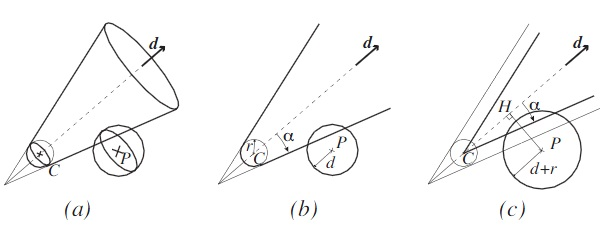
\includegraphics[scale=0.75]{Images/Node_Sphere_Intersection}
    \caption{\label{fig:crud2}Cone-Ray Union - 2D View. \small courtesy of \cite{Roger07}.}
\end{figure}

To calculate the intersection between the node, which is composed of the union of a sphere and a cone, we simplify the problem by enlarging the triangles bounding sphere \cite{Ericson04} and reducing the cones size (see Figure~\ref{fig:crud2}). The original formula for cone-sphere intersections was described in the Amanatides paper \cite{Amanatides84}. The current formula, which expands on the work of Amanatides \cite{Amanatides84}, was described by Roger et al. \cite{Roger07}.

\begin{equation}
    \mathlarger{result = {|C - H|} \times \tan{\alpha} + \frac{d+r}{\cos{\alpha}} \geqslant {|P - H|}}
\end{equation}

\subsection{Final Intersection Tests}

After traversing the hierarchy we have an array of node id and triangle id pairs. The candidates for the local intersection tests \cite{Moller97}. This final step differs according to two things, the type of ray and the depth of ray-tracing. For shadow rays all that is necessary is to indicate whether or not the ray was blocked by any other object. In contrast, for reflection and refraction rays we need to find the closest intersection and store the corresponding triangle.

\medskip

Shadow rays are only traced after tracing a batch of primary, reflection or refraction rays. As such, they use the triangles that those rays intersected instead of storing triangle intersections. Reflection and refraction rays unlike shadow rays need to store the triangle they intersected. This is necessary because after each batch of such rays we need to trace shadow rays to check whether or not the triangle has any other objects blocked its path to the light sources. 

\subsubsection{Barycentric Interpolation}

Before calculating the shading for each ray is necessary to interpolate the hit points normal in order to have smooth shading.
To interpolate the normal we use barycentric interpolation (see Figure~\ref{fig:bi}). 

\begin{figure}[!htb]
    \centering
    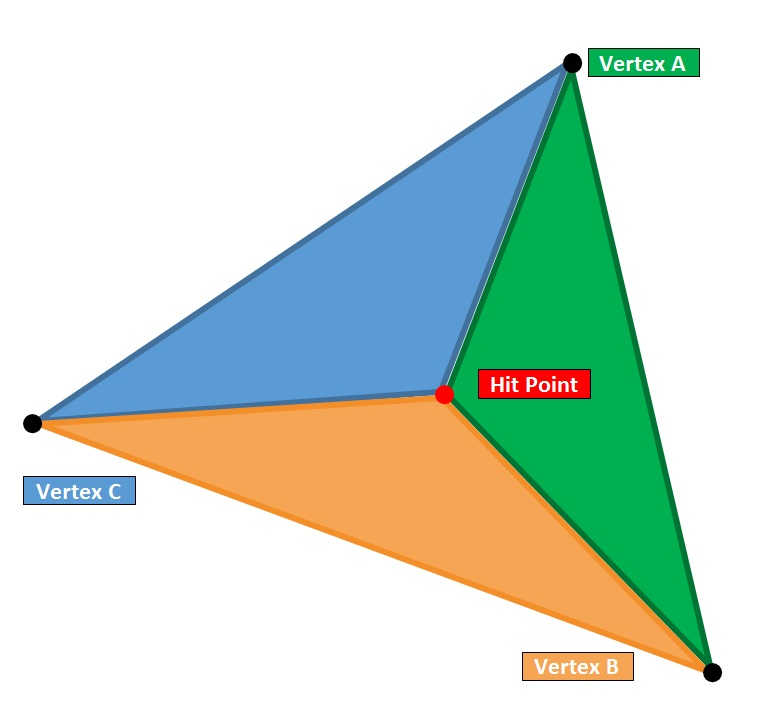
\includegraphics[scale=0.30]{Images/Barycentric_Coordinates}
    \caption{\label{fig:bi}Barycentric Coordinates.}
\end{figure}

These are the equations used to calculate the interpolated normal:

\begin{subequations}
    \begin{flalign}
        \mathlarger{area_{ABC} =} & 
        \mathlarger{\frac{(v_b - v_a) \times (v_c - v_a)}{|(v_b - v_a) \times (v_c - v_a)|}}\\[10pt]
        \mathlarger{area_{PBC} =} & 
        \mathlarger{\frac{(v_b - hitP) \times (v_c - hitP)}{|(v_b - hitP) \times (v_c - hitP)|}}\\[10pt]
        \mathlarger{area_{PCA} =} & 
        \mathlarger{\frac{(v_a - hitP) \times (v_c - hitP)}{|(v_a - hitP) \times (v_c - hitP)|}}
    \end{flalign}
\end{subequations}  

\begin{equation}
    \mathlarger{\vec{hitN} = 
        \frac{area_{PBC}}{area_{ABC}} \times n_a + 
        \frac{area_{PCA}}{area_{ABC}} \times n_b + 
        (1 - \frac{area_{PBC}}{area_{ABC}} - \frac{area_{PCA}}{area_{ABC}}) \times n_c}\\
\end{equation}  

\begin{align*}
    \textbf{hitP} = Hit Point Position,     
    \textbf{hitN} = Hit Point Normal\\
    \textbf{v\textsubscript{a}}, \textbf{v\textsubscript{b}}, \textbf{v\textsubscript{c}} = Vertex Positions,                     
    \textbf{n\textsubscript{a}}, \textbf{n\textsubscript{b}}, \textbf{n\textsubscript{c}} = Vertex Normals\\
\end{align*}

\subsubsection{Shading}

To calculate the shading we used a Lambertian reflection and Phong illumination. This is the implementation we used:

\begin{subequations}
    \begin{flalign}
        {light_{direction}} = & 
        {\frac{light_{position} - hit_{position}}{|light_{position} - hit_{position}|}}\\[10pt]
        {light_{distance} =} & 
        {|light_{position} - hit_{position}|}\\[10pt]          
        {light_{attenuation} =} & 
        {\frac{1}{att_{constant} + light_{distance} \times att_{linear} + light_{distance}^2 \times att_{exponential}}}\\[10pt]
        {view\_vector} = & 
        {\frac{hit_{position} - camera_{position}}{|hit_{position} - camera_{position}|}}\\[10pt]
        {halfway\_vector} = & 
        {\frac{light_{direction} - view\_vector}{|light_{direction} - view\_vector|}}\\[10pt]
        {diffuse\_factor} = & {\max(0,\min(1, light_{direction} \cdot hit_{normal}))}\\[10pt]
        {specular\_factor} = & {\max(0,\min(1,\max(0,halfway\_vector \cdot hit_{normal})^{shininess}))}\\[10pt]
        {color} += & {hit_{diffuse} * light_{color} * diffuse\_factor * light\_intensity * attenuation}\\[10pt]
        {color} += & {hit_{specular} * light_{color} * specular\_factor * light\_intensity * attenuation}
    \end{flalign}
\end{subequations}

In this final step all that remains is to find out which is the closest intersected triangle for each ray and accumulate shading. Depending on the depth that we want for the algorithm we might need to output another set of secondary rays. Since the algorithm is generic, all that is necessary for this is to output these rays onto the ray array that we used initially and continue from the ray compression step.